\section{Communication Protocols}
In order to establish communication between the peripherals and between different systems, there is the need to use communication protocols, depending on what are supported by these devices and what are the best in the context of the application.

%********************************* LORAWAN *************************
\subsection{LoRaWAN}
LoRa (Long Range) is a radio modulation technology for wireless LAN networks in the category of \ac{lpwa} network technologies. LoRa was developed by Cycleo and later acquired by Semtech, the founding member of LoRa Alliance, an open, non-profit association that supports the LoRaWAN protocol. LoRaWAN is a network (protocol) using LoRa. \cite{lora_alliance}

% USE THIS INSTEAD OF THE NEXT ONE????
%\begin{figure}[H]
%	\centering
%	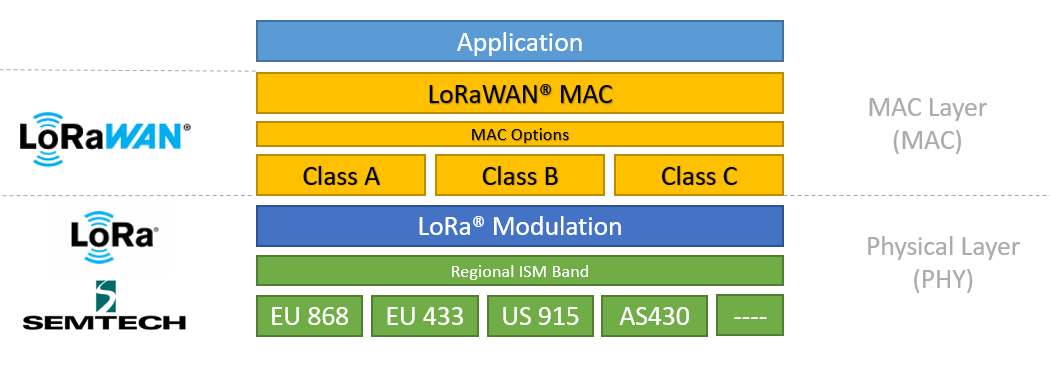
\includegraphics[width=.9\textwidth]{08theory/lora_vs_lorawan}
%	\caption{.}
%	\label{fig:lora_vs_lorawan}
%\end{figure}

LoRa technology uses the unlicensed frequency band (\ac{ism}), like 433~MHz, 868~MHz (in Europe), 915~MHz (in Australia and North America) and 923~MHz (in Asia). LoRa is the physical layer or the wireless modulation utilized to create a long range communication link, which may cover more than 10 km in line of sight. Many legacy wireless systems use \ac{fsk} modulation as the physical layer because it is a very efficient modulation for achieving low power. LoRa is based on \ac{css} modulation, which maintains the same low power characteristics as \ac{fsk} modulation but significantly increases the communication range, robustness to interference. LoRa is the first low cost implementation for commercial usage.

The LoRaWAN specification is a \ac{lpwa} networking protocol that targets key \ac{iot} requirements such as bi-directional communication, end-to-end security, mobility and localization services, whose baud rates range from 0,3~kbps to 50~kbps. LoRaWAN network architecture is deployed in a star-of-stars topology in which gateways relay messages between end-devices and a central network server. Each gateway is connected to the network server via standard IP connections, acting as a bridge by converting \ac{rf} packets to IP packets, and vice versa. The gateway only performs the forwarding of the data packets without any security protection. The end device communicates with one or more gateways by a single-hop LoRa or \ac{fsk}. LoRaWAN the protocol stack shown in figure \ref{fig:lorawan_stack}, remembering also figure \ref{fig:lora_device_classes}. \cite{what_is_lorawan}

\begin{figure}[H]
	\centering
	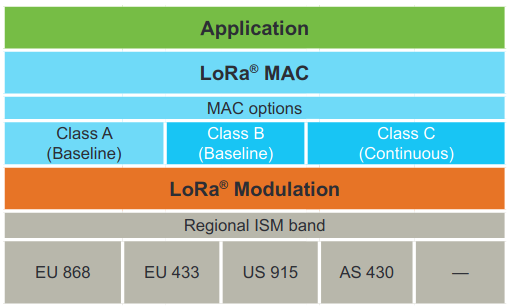
\includegraphics[width=.65\textwidth]{08theory/lorawan_stack}
	\caption{LoRaWAN protocol stack.}
	\label{fig:lorawan_stack}
\end{figure}

LoRa technology uses \ac{ism} bands, which brings vulnerability to the network. The attacker can listen on the address of the legal terminal and generate forged packets to the gateway to cause congestion. The attacker can also use his own LoRa device to send the maximum length preamble to occupy the channel maliciously. LoRaWAN considers network security issues in its design. LoRaWAN’s security policy is to encrypt data from the end device node to the network server and the application server. The former ensures that the legal node can access the network, authenticate the data packet, and perform integrity verification, and the latter ensures the end-to-end security of the application through the encryption of application data. \cite{lora_physical_layer}

\myparagraph{LoRa Frame Structure}

The LoRa frame structure is shown in figure \ref{fig:lora_packet_frame}, which comprises a preamble, an optional header and the data payload. LoRa employs two types o packet format: explicit and implicit. The explicit packet includes a short header containing information about the number of bytes, coding rate and whether a \ac{crc} is used in the packet.

\begin{figure}[H]
	\centering
	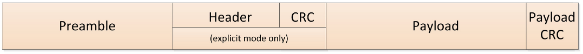
\includegraphics[width=1\textwidth]{08theory/lora_packet_frame}
	\caption{LoRa frame structure.}
	\label{fig:lora_packet_frame}
\end{figure}

The preamble is used to keep the receiver synchronized with transmitter. The packet payload is a variable-length field that contains the actual data coded at the error rate either as specified in the header  in  explicit  mode  or  in  the  register  settings  in  implicit  mode. An  optional  CRC  may  be  appended. 

%********************************* I2C *************************
\clearpage
\subsection{I2C}
The \ac{i2c} protocol is a synchronous, half-duplex, serial communication bus that uses a master-slave strategy, where the master is the device that clocks the bus, addresses slaves and writes or reads data to and from registers in slaves. I2C interface uses two-wire to allow inter-IC communication. In figure \ref{fig:i2c_interface} one can see a generalized I2C connection diagram. \cite{i2c_interface}

\begin{figure}[H]
	\centering
	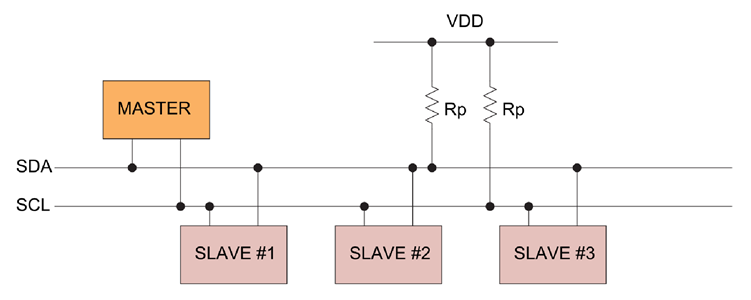
\includegraphics[width=0.8\textwidth]{08theory/i2c_interface}
	\caption{I2C configuration with master and slave devices.}
	\label{fig:i2c_interface}
\end{figure}

I2C is implemented using two lines:
\begin{itemize}
	\item \textbf{\ac{sda}}: used to send and receive data, bit by bit, between the master and slave;
	\item \textbf{\ac{scl}}: carries the clock signal, which is generated by the master device.
\end{itemize}

I2C compatible devices connect to the bus with open collector or open drain pins which pull the line LOW. When there is no transmission of data, the I2C bus lines idle in a HIGH state, being passively pulled high. Transmission occurs by toggling the lines by pulling LOW and releasing HIGH. Bits are clocked on falling clock edges. Because I2C uses addressing, multiple slaves can be controlled from a single master. With a 7 bit address, 128 ($2^7$) unique address are available. Using 10 bit addresses is uncommon, but provides 1024 ($2^{10}$) unique addresses. To connect multiple slaves to a single master, one should wire them as shown in figure \ref{fig:i2c_interface}, with 4.7 K$\Omega$ pull-up resistors, $R_{P}$, connecting the SDA and SCL lines to $V_{DD}$. \cite{i2c_basics}

\clearpage
With I2C, data is transferred in messages. Messages are broken up into frames of data. Each one are composed by the following:
\begin{itemize}
	\item \textbf{Start condition}: SDA line switches from HIGH to LOW state, before the SCL line does the same;
	\item \textbf{Stop condition}: SDA line switches from LOW to HIGH state, after the SCL line does the same;
	\item \textbf{Address frame}: 7 to 10 bit sequence that uniquely identifies the slave when the master wants to talk to it;
	\item \textbf{Read/Write bit}: bit that specifies whether the master is sending data to the slave (bit 0) or requesting data from it (bit 1);
	\item \textbf{\ac{ack}/\ac{nack} bit}: states if the address or data frame was successfully received. When successful, an ACK bit is sent, by pulling the SDA line LOW for one bit. If not, a NACK bit is sent, by leaving the SDA line HIGH.
\end{itemize}

\myparagraph{Data Transmission}

The slaves are devices that respond only when interrogated by the master, through their unique address.
\begin{enumerate}
	\item The master sends the start condition to every connected slave;
	\item The master sends each slave the address frame of the slave it wants to communicate with, along with the read/write bit;
	\item Each slave compares the address sent from the master to its own address. If they match, the slave returns an \ac{ack} bit. Else, the slave leaves the SDA line HIGH;
	\item The master sends or receives the data frame;
	\item After each data frame has been transferred, the receiving device returns another ACK bit to the sender, to acknowledge successful receipt of the frame;
	\item To stop the data transmission, the master sends a stop condition to the slave.
\end{enumerate}

I2C has advantages comparing to other communication protocols. I2C uses only two wires, and supports multiple masters and multiple slaves and ACK/NACK bit gives confirmation that each frame is transferred successfully. However, this protocol has slower data transfer rate than SPI, for example, the size of the data frame is limited to 8 bits and has more complicated hardware to implement than SPI.

%********************************* SPI *************************
\clearpage
\subsection{SPI}
The \ac{spi} protocol is a synchronous, full-duplex, serial communication interface that uses a master-slave strategy, where a microcontroller takes the role of the master. SPI interfaces can have only one master and can have one or multiple slaves. SPI interface can be either 3-wire or 4-wire interface. One will focus in the popular 4-wire SPI interface, as one can see in figure \ref{fig:spi_interface}. \cite{spi_interface}

\begin{figure}[H]
	\centering
	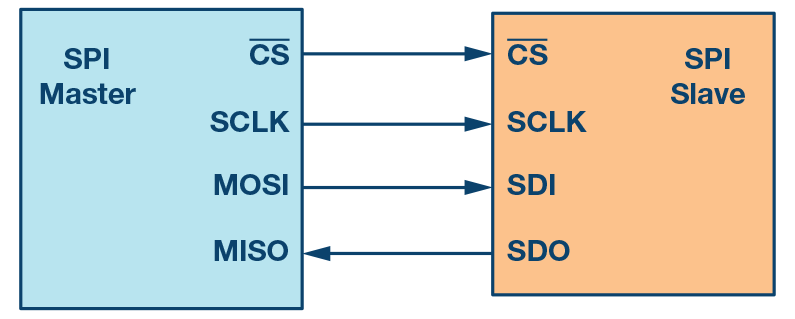
\includegraphics[width=0.6\textwidth]{08theory/spi_interface}
	\caption{SPI configuration between master and slave devices.}
	\label{fig:spi_interface}
\end{figure}

4-wire SPI devices makes use of four signals:
\begin{itemize}
	\item \textbf{Clock (SPI CLK or SCLK)}: generated by the master device, and used to synchronize the data transmitted between the master and the slave;
	\item \textbf{Chip Select (CS)}: signal that comes from the master and is used to select the slave. When multiple slaves are used, an individual CS for each slave is required from the master;
	\item \textbf{\ac{mosi}}: data line to transmit data from the master to the slave;
	\item \textbf{\ac{miso}}: data line to transmit data from the slave to the master.
\end{itemize}

\myparagraph{Data Transmission}

In this protocol both master and slave devices have an internal shift register, controlled by the clock signal generated by the master.
\clearpage
The steps of SPI data transmission are the following:

\begin{enumerate}
	\item To begin SPI communication, the master must send the clock signal;
	\item The master selects the slave by enabling the CS signal, by a low voltage state;
	\item The master sends the data one bit at a time to the slave, using the \ac{mosi} line. The slave reads the bits as they are received;
	\item If a response is needed, the slave returns data, one bit at a time, to the master, using the \ac{miso} line. The master reads the bits as they are received.
\end{enumerate}

SPI has advantages comparing to other communication protocols. It doesn't have start and stop bits, do the data can be streamed continuously without interruption. It is full-duplex, having separate lines for receiving and sending data. Has higher data transfer rate and has a simpler slave addressing system than I2C. However, this protocol uses four wires, in contrast to two used by I2C, has no acknowledgment that the data has been successfully received and only allows for a single master. \cite{spi_basics}

%********************************* CSI *************************
\clearpage
\subsection{CSI}
The \ac{csi} is a specification of the \ac{mipi} Alliance. It is a widely adopted, simple, high-speed protocol primarily intended for point-to-point image and video transmission between a camera and a host processor. The latest active interface specifications are CSI-2 v3.0, CSI-3 v1.1 which were released in 2019 and 2014 respectively. \cite{csi_basics}

The CSI-2 is the most widely used camera interface in mobile and other markets. CSI-2 consists of a unique physical bus that contains a differential clock, source synchronous, and from one to four differential data lanes, as one can see in figure \ref{fig:csi_interface}. This interface is called a D-PHY. This standard takes advantage of \ac{lvds} to send data through multiple lanes from the camera controller to the MIPI. The LVDS standard is used to reduce electromagnetic interference and cross talk between lanes.

\begin{figure}[H]
	\centering
	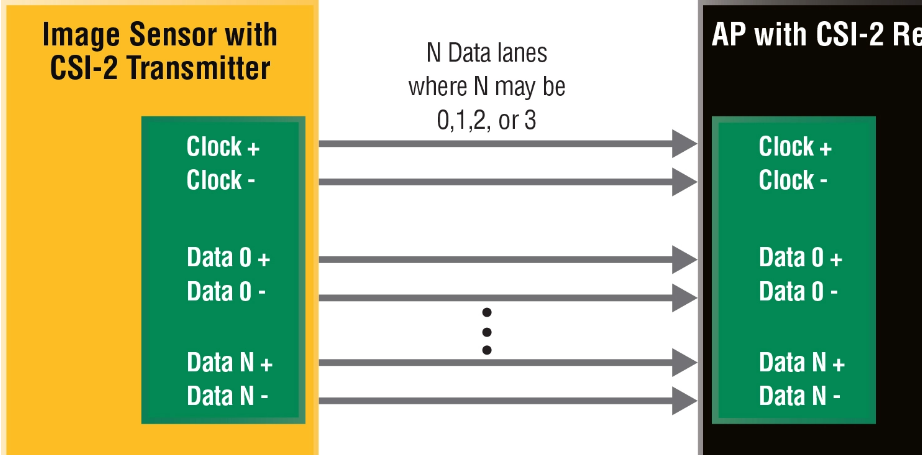
\includegraphics[width=0.7\textwidth]{08theory/csi_interface}
	\caption{CPI-2 sensor interface.}
	\label{fig:csi_interface}
\end{figure}

Each data lane transmits 8-bit serial data. The higher the image sensor resolution and frame rate, the more data lanes and higher speed for each will be required. The practical limit for a CSI-2 interface is less than 1 Gbits/s data rates, but often it is less than 700 Mbits/s. \cite{csi_interface}

%********************************* TCP-IP *************************
\clearpage
\subsection{TCP-IP}
\ac{tcp}/\ac{ip} is one of the most commonly used protocols for internet communication. TCP is the component that collects and reassembles the packets of data, while IP is responsible for making sure the packets are sent to the right destination. These are part of the OSI model, as shown in figure \ref{fig:osi_model}.

\begin{figure}[H]
	\centering
	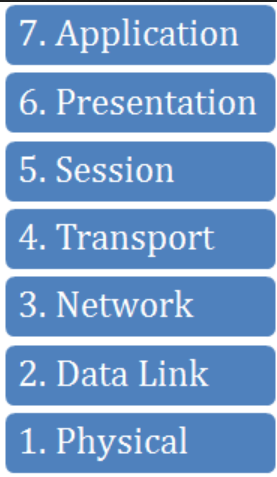
\includegraphics[width=0.3\textwidth]{08theory/osi_model}
	\caption{OSI model.}
	\label{fig:osi_model}
\end{figure}

The TCP provides services to the transport layer, providing a reliable and sequenced delivery of data. One can compare TCP to while the \ac{udp} provides data transportation without guaranteed data delivery or acknowledgments, which may be faster, but unreliable on the other hand. The IP part of the TCP/IP protocol, provides services to the network layer, and is used to make origin and destination addresses available to route data across networks.

\clearpage
\myparagraph{Creating a TCP Server}

In order to create a TCP server, one needs to perform the following steps:
\begin{enumerate}
	\item Create a TCP socket, using \textit{create()};
	\item Bind the created socket to a server address, using \textit{bind()};
	\item Using \textit{listen()}, put the server socket in a passive mode, waiting for the client to approach the server to make a connection;
	\item Establish a connection, between client and server, using \textit{accept()}; Both can now transfer data;
	\item Go back to step 3, to listen for more client connections.	
\end{enumerate}

\myparagraph{Creating a TCP Client}

In order to create a TCP client, one needs to perform the following steps:
\begin{enumerate}
	\item Create a TCP socket;
	\item Connect newly created client socket to server, using \textit{connect()};
\end{enumerate}

%********************************* HTTP *************************
\clearpage
\subsection{HTTP}
\ac{http} is a protocol for fetching resources such as HTML documents. It is the foundation of any data exchange on the Web and it is a client-server protocol, which means requests are initiated by the recipient, usually the Web browser. A complete document is reconstructed from the different sub-documents fetched, for instance, text, layout description, images, videos, scripts, and more. \cite{http}

Clients and servers communicate by exchanging individual messages (as opposed to a stream of data). The messages sent by the client, usually a Web browser, are called \textit{requests} and the messages sent by the server as an answer are called \textit{responses}. It is an application layer protocol that is sent over TCP, though any reliable transport protocol could theoretically be used. 

Each individual request is sent to a server, which handles it and provides an answer called the response. Between the client and the server there are numerous entities, collectively called proxies, which perform different operations and act as gateways or caches, for example, as shown in figure \ref{fig:http}.

\begin{figure}[H]
	\centering
	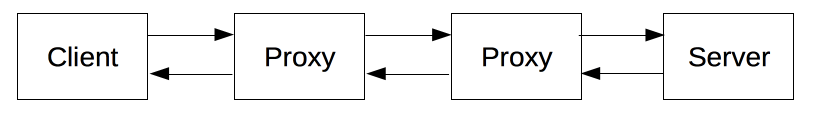
\includegraphics[width=0.8\textwidth]{08theory/http}
	\caption{Components of HTTP-based systems.}
	\label{fig:http}
\end{figure}

\myparagraph{Client-Server Communication}

When a client wants to communicate with a server it performs the following steps:
\begin{enumerate}
	\item Open a TCP connection, which is used to send a request or to receive an answer;
	\item Send an HTTP message;
	\item Read the response sent by the server;
	\item Close or reuse the connection for further requests;
\end{enumerate}

If HTTP pipelining is activated, several requests can be sent without waiting for the first response to be fully received.

\myparagraph{HTTP Request methods}

HTTP defines a set of request methods to indicate the desired action to be performed for a given resource. Below are listed some of the HTTP request methods. \cite{http_methods}

\begin{itemize}
	\item \verb|GET|: requests a representation of the specified resource;
	\item \verb|HEAD|: asks for a response identical to a \verb|GET| request, but without the response body;
	\item \verb|POST|: submits an entity to the specified resource;
	\item \verb|PUT|: replaces all current representations of the target resource with the request payload;
	\item \verb|DELETE|: deletes the specified resource;
\end{itemize}

\myparagraph{HTTP Messages}

HTTP messages are human-readable, having two types of messages, requests and responses, each with its own format.\\

\textbf{Requests} consists of the following elements:
\begin{itemize}
	\item HTTP method, that defines the operation the client wants to perform: usually a verb like \verb|GET|, \verb|POST| or a noun like \verb|OPTIONS| or \verb|HEAD|.
	\item Path of the resource to fetch: the URL of the resource stripped from elements that are obvious from the context;
	\item The version of the HTTP protocol using;
	\item Optional headers, conveying additional information for the servers;
	\item A body for some methods like \verb|POST|, which contains the resource sent.
\end{itemize}

\clearpage
\textbf{Responses} consists of the following elements:
\begin{itemize}
	\item The version of the HTTP protocol using;
	\item Status code, indicating if the request was successful or not, and why;
	\item Status message: a non-authoritative short description of the status code;
	\item HTTP headers;
	\item Optionally a body containing the fetched resource.
\end{itemize}
%\subsection{MQTT}